
We developed a compiler that compiles programs to byte-code and a multi-threaded
virtual machine (VM) using the Pthreads library that runs the byte-code.
If we execute programs with $P$ threads, our implementation will partitions the application
graph of $N$ nodes into $P$ subgraphs and then each thread will work on their own subgraph.
The goal of our system is to keep the threads as busy as possible and to reduce inter-thread communication.

The load balancing aspect of the system is performed by our work scheduler that is based on a work
stealing algorithm. More specifically, threads can steal nodes of other threads to keep themselves busy.

Reduction of inter-thread communication is achieved by first ordering the node addresses present
in the code in such a way that closer nodes are clustered together and then partitioning them
to threads.
During compilation, we take note of predicates that are used in rules for
communication rules (arguments with type \emph{node}) and then build a graph of nodes from
the program's axioms. The nodes of the graph are then ordered by using a breadth-first search
algorithm that changes the nodes of addresses to the domain $[0, n[$, where $n$ is the number of
nodes. Once the VM starts, we simply partition the range
$[0, n[$.

\subsubsection{Multicore}

When the VM starts, it reads the byte-code file and starts all threads.
As a first step, all threads will grab their nodes and assign the \texttt{owner} property of each node.
Because only one thread is allowed to do computation on a node at any giving time, the owner property
defines the thread with such permission.
Next, each thread fills up its \emph{work queue} with the initial nodes. This queue
maintains the nodes that have new facts to be processed.

The main thread loop is shown in Fig.~\ref{code:work_loop}, where the threads
inspects their work queue for active nodes. Procedure \texttt{process\_node} takes a node with new candidate rules
and executes them. If the work queue is empty, the thread attempts to steal one node from another thread before
becoming idle. Starting from a random thread, it cycles through all the threads to find one active node.

\begin{figure}[h!]
   \vspace{-0.5\intextsep}
\scriptsize\begin{Verbatim}
void work_loop(thread_id tid):
   while (true):
      if(has_work(tid)):
         current_node = pop_work(tid); // take node from the queue
      else:
         for (i = 0; i < NUM_THREADS; ++i): // need to steal a node
            if (current_node = steal_node_from_thread(target_thread):
               break;
            target_thread = (target_thread + 1) % NUM_THREADS;
      if(current_node == NULL):
         become_idle(tid);
         if(!synchronize_termination(tid)):
            return;
         become_active(tid);
      else:
         process_node(current_node, tid);
\end{Verbatim}
\vspace{-0.5\intextsep}
  \caption{Thread work loop.}
  \label{code:work_loop}
  \vspace{-0.5\intextsep}
\end{figure}

When a node sends a fact to another node, we need to check if the target node is owned by the same thread.
If that is not the case, then we have a point of synchronization and we may need to
make the target thread active.

Eventually, there will be no more work to do and the threads will go idle. There is a global atomic counter, a global
boolean flag and one boolean flag for each thread that are used to detect termination.
Once a thread goes idle, it decrements the global counter and changes its flag to idle. If the counter
reaches zero, the global flag is set to idle. Since every thread will be busy-waiting and checking
the global flag, they will detect the change and exit the program.

\subsubsection{Byte-Code}

A byte-code file contains meta-data about the program's predicates, initial nodes, partitioning
information, and code for each rule. Rule code uses a custom-made set of instructions that
use the database to match the body of the rule and then derive the head. Note that a rule
is only executed if there is a good change that it will successfully match (more details
in "Rule Engine").

Each VM thread has 32 registers that are used during rule execution.
Registers can store facts, integers, floats, node addresses and pointers to runtime 
data structures (lists and structures). When registers store facts, we can reference
fields in the fact through the register.

Consider a rule \texttt{!a(X,Y), b(X,Z), c(X,Y) -o d(Y)} and a database with
\texttt{!a(1,2)}, \texttt{!a(2,3)}, \texttt{b(1,3)}, \texttt{b(5,3)}, \texttt{c(1,2)}, \texttt{c(1,3)},
\texttt{c(5,3)}. Rule execution proceeds in a series of recursive loops, as follows: the first loop retrieves an
iterator for the persistent facts of \texttt{!a/2} and moves the first valid fact, \texttt{!a(1,2)},
to register 0; the inner loop retrieves linear facts that match \texttt{b(1,Z)} (from the
\emph{join constraint}) and moves \texttt{b(1,3)} to register 1; in the final
loop we move \texttt{c(1,2)} to register 2 and the body of the rule is successfully matched. Next, we
derive \texttt{d(2)}, where \texttt{2} comes from register 0.
Fig.~\ref{fig:byte_code} shows the byte-code for this example.

\begin{wrapfigure}{l}{0.45\textwidth}
   \vspace{-1\intextsep}
\scriptsize\begin{Verbatim}
PERSISTENT ITERATE a MATCHING TO reg 0
  LINEAR ITERATE b MATCHING TO reg 1
      (match).0=0.0
    LINEAR ITERATE c MATCHING TO reg 2
        (match).0=0.0
        (match).1=0.1
      ALLOC d TO reg 3
      MVFIELDFIELD 0.1 TO 3.0
      ADDLINEAR reg 3
      REMOVE reg 2
      REMOVE reg 1
      RETURN DERIVED
    NEXT
  NEXT
RETURN
\end{Verbatim}
\caption{\small{Byte-code for rule \texttt{!a(X,Y), b(X,Z), c(X,Y) -o d(Y).}}}
\label{fig:byte_code}
\vspace{-1\intextsep}
\end{wrapfigure}

In case of failure to find a valid fact at any given loop, we jump
to the outer loop in order to try the next candidate.
If a rule match succeeds and the head is derived, we backtrack to the inner most valid loop:
if any loop uses linear facts we remove the fact from the database, but we will
continue backtracking until we reach the first loop that uses linear facts,
because all the others are now invalid (invalid candidates). In our example, we would jump to the
loop of \texttt{b(X,Z)} and not \texttt{c(X,Y)}, since \texttt{b(1,3)} was already consumed.

The compiler re-orders the fact expressions used in the body in order to make execution more
efficient. For example, it forces the join constraints in rules to appear at the beginning so
that matching will fail sooner rather than later. It also does the same for constraints.
Note that for every loop, the compiler adds a \emph{match object}, which contains information
about which arguments need to match, so that runtime matching is efficient.

\subsubsection{Database Data Structures}\label{sec:database}

We said before that LM rules are constrained by the first argument. Because nodes can execute
independently, our database is indexed by the node address and each sub-database does not
need to deal with synchronization issues since at any given point, only one thread will be using
the database. Note that the first argument of each fact is not stored.

Each (sub-)database is implemented using three data structures: trie data structures, list data structures and hash table data structures.
The database must be implemented efficiently because during matching of rules we need
to restrict the facts using a given match object, which fixes arguments of the target predicate to instantiated values. The data structures used are as follows:

\begin{itemize}
   \item \emph{Trie Data Structures} are used exclusively to store persistent facts.
   Tries are trees where facts are indexed by the common arguments.
      
   \item \emph{Doubly Linked List Data Structures} are used to store linear facts.
   Each fact contains the standard \texttt{prev} and \texttt{next} pointers
   and the fact arguments. We use a double linked list because it is very efficient to add and remove facts.
   
   \item \emph{Hash Table Data Structures} are used when linked lists are too long and we need to search filter by a fixed argument. The virtual machine decides which arguments are best to be indexed
   (see "Indexing") and then
   uses an hash table indexed by the appropriate argument. If we need to go through all the facts, we just iterate through all the facts in the table. For collisions, we use the above doubly linked list data structure.
\end{itemize}

\begin{wrapfigure}{r}{0.5\textwidth}
   \vspace{-1\intextsep}
   \centering
   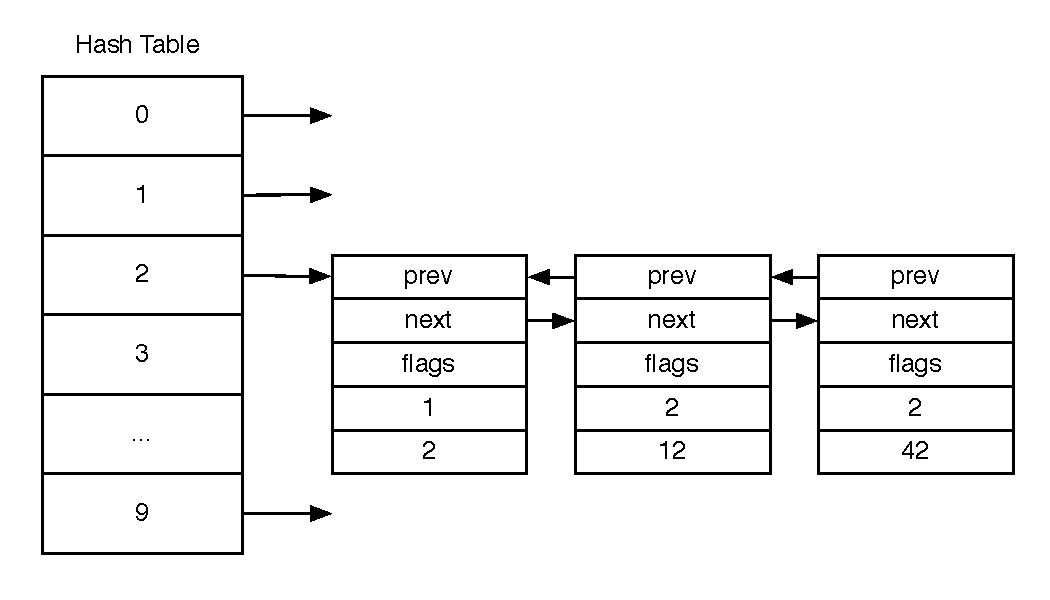
\includegraphics[width=0.48\textwidth]{hash_table.pdf}
   \caption{Example hash table data structure for storing predicate \texttt{a(int,int)}.}
   \label{fig:hash_table}
   \vspace{-0.5\intextsep}
\end{wrapfigure}

In Fig.~\ref{fig:hash_table} we show an example hash table data structure storing predicate \texttt{a(int,int)}. The table
has 10 buckets and indexes facts by the second argument. We show the doubly linked list for bucket \texttt{2}. Each linear fact
contains the regular list pointers, the fact arguments and a \texttt{flags} field. Those are all stored continuously to improve data
locality. One use of the \texttt{flags} field is to mark that a fact is already being used. For example,
consider the rule body \texttt{a(A,B), a(C,D) -o ...}. We first pick a fact for \texttt{a(A, B)} from the hash table, then we mark it as
being used and when we retrieve facts for \texttt{a(C, D)}, we know that one of them cannot be used because it would
violate linearity.

\subsubsection{Rule Engine}\label{rule_engine}

The rule engine decides which rules may need to be executed while taking into account rule priorities.
In Fig.~\ref{fig:rule_engine} we present the 5 main data structures for scheduling rule execution.
\texttt{Rule Queue} is the bitmap representing the rules that will be run, \texttt{Active Bitmap} contains the rules that have enough
facts to be fired, \texttt{Inactive Bitmap} contains the rules that must be dropped from \texttt{Rule Queue}, \texttt{Predicates Bitmap}
marks the newly derived facts and \texttt{Predicates Count} counts the number of facts per predicate.
To understand how our engine works, consider
the program in Fig.~\ref{code:5rules}.

\begin{wrapfigure}{l}{0.3\textwidth}
\vspace{-0.5\intextsep}
\footnotesize\begin{Verbatim}
a, e(1) -o b.
a -o c.
b -o d.
e(0) -o f.
c -o e(1).
\end{Verbatim}
\vspace{-.5\intextsep}
\caption{\small{Example program with 5 rules.}}
\label{code:5rules}
\vspace{-0.8\intextsep}
\end{wrapfigure}

We take the least significant rule from \texttt{Rule Queue}, which is the candidate rule with the higher priority, and then run it. In our example, we need to execute the second rule \texttt{a -o c}, since we have facts \texttt{a} and \texttt{e(0)}.
Because the derivation is successful, we derive \texttt{c} and consume \texttt{a}. In Fig.~\ref{fig:rule_engine}~(b) we
activate the \texttt{c} predicate in the \texttt{Predicates Bitmap} since it was derived and then activate the first and second rules
in \texttt{Dropped Bitmap} since such rules are no longer applicable (\texttt{a} is gone). To update the \texttt{Rule Queue},
we remove the bits marked in \texttt{Dropped Bitmap} and add the active rules marked in \texttt{Active Bitmap} that are affected
by predicates in \texttt{Predicates Map}. The engine thus schedules the fourth and fifth rules to run.

Note that every node in the program has the same set of data structures present in Fig.~\ref{fig:rule_engine}.
We use 32 bits integers to implement bitmaps and an array of 16 bits integers to count facts, resulting in
$32 + 2P$ bytes per predicate.

We do a small optimization to reduce the number of derivations of persistent facts. We
divide the program rules into two sets: \emph{persistent rules} and \emph{non persistent rules}.
Persistent rules are rules where only persistent facts are involved. We compile such rules
incrementally, that is, we attempt to fire all rules where a persistent fact is used. This is called
the \emph{pipelined semi-naive} evaluation and it originated in the P2 system~\cite{Loo-condie-garofalakis-p2}.
This evaluation method avoids excessing re-derivations of the same fact. The order of derivation does not matter for those rules, since
only persistent facts are used.

\begin{figure*}[h]
   \vspace{-\intextsep}
   \centering
   \begin{subfigure}[b]{0.45\textwidth}
      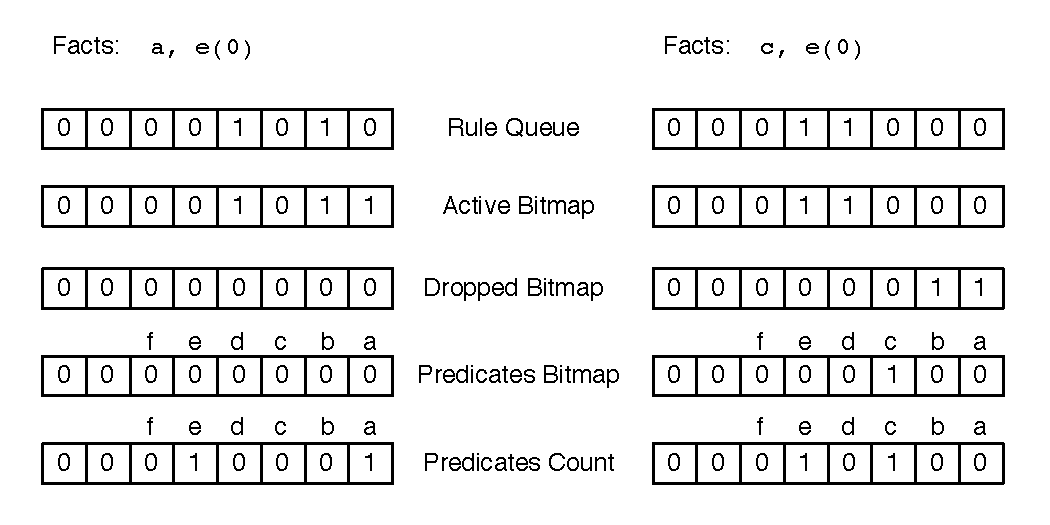
\includegraphics[width=\textwidth]{rule_queue1.pdf}
      \caption{Before applying the second rule.}
   \end{subfigure}
   \begin{subfigure}[b]{0.45\textwidth}
      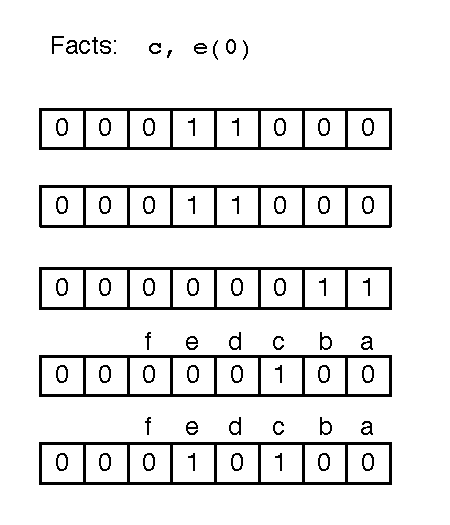
\includegraphics[width=\textwidth]{rule_queue2.pdf}
      \caption{After applying the second rule.}
   \end{subfigure}
   \caption{Rule engine main data structures.}
   \label{fig:rule_engine}
   \vspace{-1.5\intextsep}
\end{figure*}

\paragraph{Thread Interaction}

Whenever a node derives a new fact through rule derivation, we need to update the data structures of the rule engine.
This is trivial if done by the thread that owns the node, however, if a thread $T1$ executes a node and a fact is derived
at a node owned by another thread $T2$, then we may have problems because $T2$ may be also updating the data structures.
We added a lock and a boolean flag to each node to protect the access to the data structures. When a node starts to execute,
we activate the flag and lock the node. When another thread tries to use the data structures, if first checks the flag and if
not activated, it locks the node and performs the required updates. If the flag is activated, it stores the new fact
in a list to be processed before the node is executed.

\subsubsection{Indexing}\label{indexing}

In Section~\ref{rule_engine} we explained that we use hash tables to dynamically index facts.
The VM employs a fully dynamic mechanism to decide which argument may be optimal to improve fact lookup.
The algorithm is performed in the initial part of the program execution and empirically tries to assess the argument
of each predicate that more equally spreads the database across the values of the argument. Note that only one thread
performs the algorithm.

The indexing algorithm is performed in three main steps. First, it gathers statistics of lookup data by keeping a counter
of each predicate's argument.
Every time a fact search is performed where arguments are fixed to a value, the counter of such arguments is incremented. This phase is performed during rule execution of $1/25n$ nodes, where $n$ is the number of nodes in the program.

The second step of the algorithm initially decides the candidate arguments of each predicate.
If a predicate did not fix any arguments, then it will be not indexed.
If only one argument was fixed, then such such argument is set as the indexing argument. Otherwise, the top 2 arguments
are selected for the third phase, where \emph{entropy statistics} are collected dynamically.

During the third phase, each candidate argument has an entropy score.
Before a node is executed, the facts of the target predicate
are used in the following formula applied for the two arguments:

\vspace{-0.5\intextsep}

\[
Entropy(A, F) = - \sum_{v \in values(F, A)} \frac{count(F, A = v)}{total(F)} 	\log_2 \frac{count(F, A = v)}{total(F)}
\]
\vspace{-0.5\intextsep}

Where $A$ is the target argument, $F$ is the multi-set of linear facts for the target predicate, $values(F, A)$ is set of values of the argument $A$, $count(F, A = v)$ counts the number
of linear facts where argument $A$ is equal to $v$ and $total(F)$ counts the number of linear facts in $F$.
The entropy value is a good metric because it tells us how much information is needed to describe an argument.
If more information is needed, then that must be the best argument to index.

For one of the arguments to score, $Entropy(A, F)$ multiplied by the number of times it has been used for lookup must be larger than the other argument. This is performed for $1/25n$ node executions.

In the final and third phase, the best argument with the best score is selected and then
a global variable called \texttt{indexing\_epoch} is updated.
In order to convert the node's linked lists into hash tables, each node has local variable also called \texttt{indexing\_epoch}
that is compared to the global variable in order to rebuild the node database according to the new indexing
information.

Our VM also dynamically resizes the hash table to accommodate every increasing or decreasing hash tables. When the hash table becomes
too dense, the hash table becomes twice as big. When it becomes too sparse, the table is reduce in half
or simply transformed back into a doubly linked list. This is done once in a while, before a node executes.

In our experience, we have seen very good results with this scheme, with programs such as the all-pairs shortest paths with a 2 to 5-fold
improvement in speed. The overhead of dynamic indexing is also negligible since programs run almost as fast
as if the indices have been added from the start.

\begin{wrapfigure}{r}{0.5\textwidth}
\vspace{-1.5\intextsep}
\scriptsize\begin{Verbatim}
LINEAR ITERATE a MATCHING TO reg 0
  MVFIELDREG 0.0 TO reg 1
  MVINTREG INT 1 TO reg 2
  reg 1 INT PLUS reg 2 TO reg 3
  MVREGFIELD reg 3 TO 0.0
  UPDATE reg 0
  RETURN DERIVED
RETURN
\end{Verbatim}
\vspace{-0.5\intextsep}
\caption{\small{Byte-code for rule \texttt{a(N) -o a(N+1)}.}}
\label{code:update}
\vspace{-1.3\intextsep}
\end{wrapfigure}

\subsubsection{Update Optimization}

Our compiler also detects cases where we re-derive a linear fact with new arguments.
For example, as shown in Fig.~\ref{code:update}, the rule \texttt{a(N) -o a(N+1)}
will compile to code that reuses the old \texttt{a(N)} fact.
We use the \texttt{flags} field presented in Section~\ref{sec:database} to mark updated nodes.

\iffalse

\subsubsection{Runtime Data Structures}

LM supports recursive types such as lists and pairs. These complex data structures are stored in
the heap of the VM and are managed through reference counting. For instance, each list
is a \emph{cons cell} with 3 fields: \texttt{tail}, the pointer to the next element of the list;
\texttt{head}, the element stored by this element of the list; and \texttt{refs} that counts the
number of pointers to this list element in the VM. The list is deleted from the heap whenever
\texttt{refs} is decremented to 0.

\fi